\documentclass{beamer}

\usepackage[english]{babel}
\usepackage{minted}
\newcommand{\mil}[1]{\mintinline{java}{#1}}
\usepackage{upquote}
\usepackage{graphicx}
\usepackage{tikz}
\usetikzlibrary{matrix,backgrounds}
\usepackage{hyperref}

\title[Layouts]{JavaFX}
\subtitle{Layouts} % (optional)

\author[]{Dalton State College} 

%\institute[Dalton State College]

\date[T. Gonzalez]{T. Gonzalez}

% If you wish to uncover everything in a step-wise fashion, uncomment
% the following command: 

%\beamerdefaultoverlayspecification{<+->}


\begin{document}

\begin{frame}

	\titlepage
	
\end{frame}

\begin{frame}
    
    \frametitle{Scene Graph}
    
    A \textbf{scene graph} is a diagram that shows the containment relationships among all components in a scene.
    
    \bigskip
    
    \begin{center}
        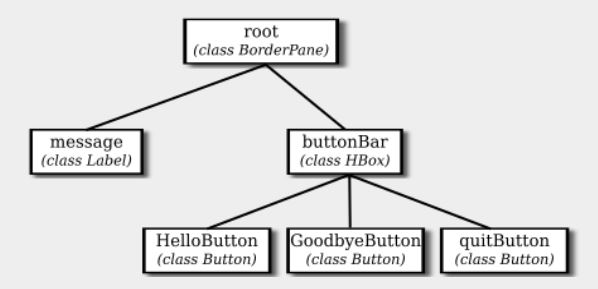
\includegraphics[scale=0.5]{scene_graph.jpg}
    \end{center}
    
\end{frame}

\begin{frame}[fragile]

	\frametitle{Nodes}
	
    The components that can be in a scene (and hence a scene graph) are referred to as \textbf{nodes}.
    
    \bigskip
    
    Nodes are child classes of \mil{javafx.scene.Node}.
    
    \bigskip
    
    Nodes that can act as containers must be child classes of \mil{javafx.scene.Parent} which is a child class of \mil{Node}.
    
    \bigskip
    
    The nodes contained in a container are called \textbf{children} of that node.
	
\end{frame}

\begin{frame}[fragile]

	\frametitle{Scene Graph Implementation}
	
	See SceneGraphImplementation.java.  

\end{frame}
	


\begin{frame}

    \frametitle{Layout}
    
    A layout is a positioning of GUI components in a scene.  
    
    \bigskip
    
    Positions and sizes for each component must be determined.
\end{frame}



\begin{frame}

    \frametitle{Containers and Nodes}
    
    The layout of the child nodes is usually done automatically by the container.
    
    \bigskip
    
    Different containers have different ways for laying out their child nodes.
    
    \bigskip
    
    Every node has a minimum width and height, a maximum width and height, and a preferred width and height.
    
    \bigskip
    
    Containers usually consults these values when laying out its children.
    
    \bigskip
    
    Containers will compute its own preferred size based on the nodes it contains, allowing each child node to have at least its preferred size, and similarly for minimum and maximum sizes.
    
    \bigskip
    
    Resizable nodes, such as controls and most containers, have methods for changing preferred, minimum, and maximum sizes.
\end{frame}

\begin{frame}
    
    \frametitle{Layouts}
    
    In JavaFX, containers that do layouts are \mil{javafx.scene.layout.Pane} and its child classes.
    
\end{frame}

\begin{frame}

    \frametitle{\mil{Pane}}
    
    Add nodes to a \mil{Pane} by calling \mil{getChildren().add()} or \mil{addAll()}.
    
    \bigskip
    
    Use the \mil{relocate()} method to set the position of a node by specifying an x and y coordinate.
    
    \bigskip
    
    Use the \mil{resize()} method to set the width and height of a resizable node.
    
    \bigskip
    
    Before the \mil{resize()} method will work, the node must call \mil{setManaged(false)}.
    
    \bigskip
    
    See PaneDemo.java.
\end{frame}

\begin{frame}
    
    \frametitle{\mil{BorderPane}}
    
    \mil{BorderPane} lays out its children in top, left, right, bottom, and center positions.
    
    \begin{center}
        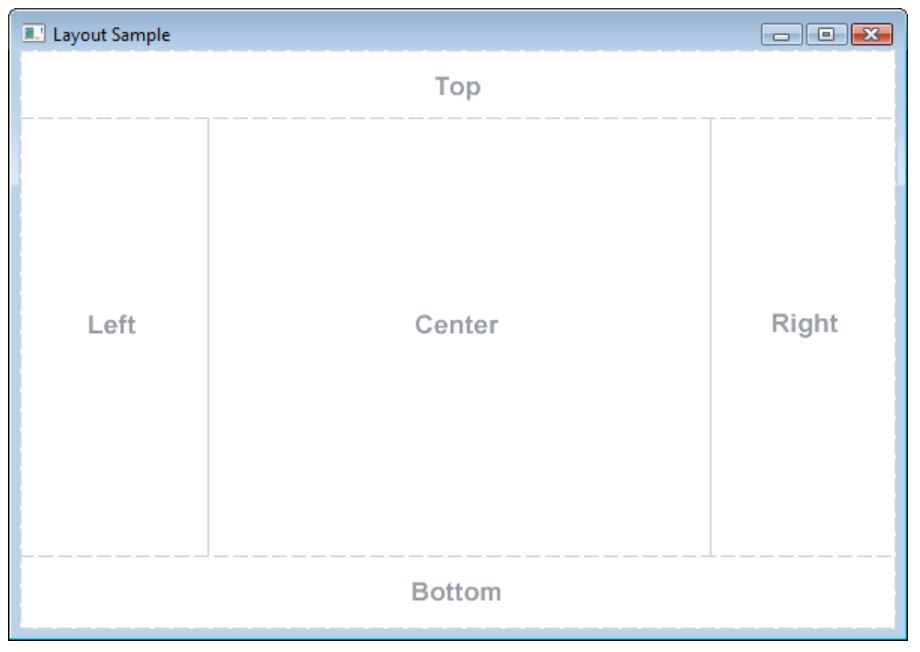
\includegraphics[scale=0.4]{borderpane.jpg}
    \end{center}
        
\end{frame}

\begin{frame}

    \frametitle{Adding Children to \mil{BorderPane} Compartments}
    
    Use the following methods to add child nodes to the \mil{BorderPane} compartments:
    
    \begin{itemize}
        \item \mil{setTop()}
        \item \mil{setBottom()}
        \item \mil{setLeft()}
        \item \mil{setRight()}
        \item \mil{setCenter()}
    \end{itemize}
    
    \bigskip
    
    Use these methods with \mil{null} as the argument to remove the child node.
\end{frame}

\begin{frame}
    
    \frametitle{Alignments}
    
    Nodes can be aligned within \mil{BorderPane} compartments by using the \mil{static} method call
    
    \bigskip
    
    \mil{BorderPane.setAlignment( child, position);}
    
    \bigskip
    
    The position can be any of the values in the \mil{javafx.geometry.Pos} class.
    
    \bigskip
    
    See the documentation for \mil{javafx.geometry.Pos}.
    
    \bigskip
    
    See BorderPaneDemo.java.
    
\end{frame}

\begin{frame}
    
    \frametitle{\mil{HBox}}
    
    \mil{HBox} lays out it nodes in a horizontal row.
    
    \bigskip
    
    Use the \mil{setSpacing()} method to increase the spacing between nodes.
    
    \bigskip
    
    Use the \mil{getChildren().add()} or \mil{addAll()} method to add child nodes.
\end{frame}

\begin{frame}
    
    \frametitle{\mil{VBox}}
    
    \mil{VBox} lays out it nodes in a vertical column.
    
    \bigskip
    
    Use the \mil{setSpacing()} method to increase the spacing between nodes.
    
    \bigskip
    
    Use the \mil{getChildren().add()} or \mil{addAll()} method to add child nodes.    
\end{frame}

\begin{frame}
    
    \frametitle{\mil{GridPane}}
    
    \mil{GridPane} uses a grid to layout its child nodes in rows and columns.
    
    \begin{center}
        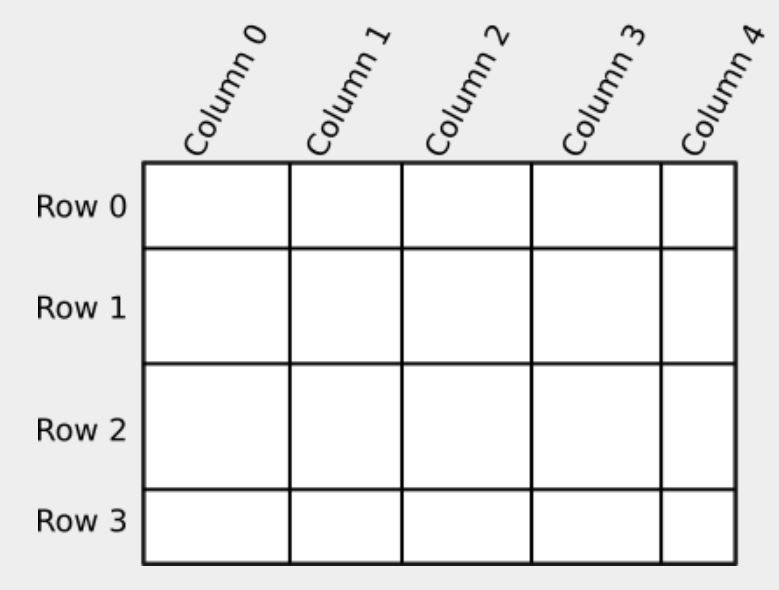
\includegraphics[scale=0.4]{gridpane.jpg}
    \end{center}
\end{frame}

\begin{frame}
    \frametitle{Adding Nodes to \mil{GridPane}}
    
    \mil{root.add( child, column, row );}
    
    \bigskip
    
    \mil{root.add( child, column, row, colspan, rowspan);}
    
    \bigskip
    
    See GridPaneDemo.java
    
\end{frame}

\begin{frame}
    
    \frametitle{\mil{TilePane}}

    \mil{TilePane} lays out its children in a grid of uniformly sized tiles.
    
    \bigskip
    
    See TilePaneDemo.java.
        
\end{frame}

\begin{frame}
    
    \frametitle{\mil{FlowPane}}

    \mil{FlowPane} lays out its children in a grid of tiles.  The size of the tiles does not have to be uniform.
    
    \bigskip
    
    See FlowPaneDemo.java.
        
\end{frame}

\begin{frame}
    \frametitle{In-Class Problem}
    
        \begin{center}
    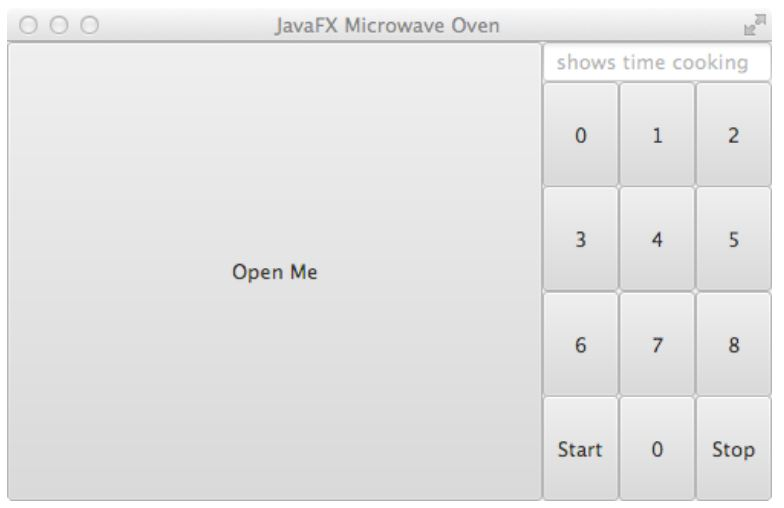
\includegraphics[scale=0.4]{microwave_oven.jpg}
    \end{center}
    
\end{frame}
\end{document}